\chapter{SPEXS Generalization}
\label{c:generalization}

\WIP

In this chapter we show how to make SPEXS algorithm more abstract by allowing flexibilty through function composition and finding minimal requirements for the data-structures.

\section{Algorithm}

The algorithm in a more conventional view is:

\begin{algorithm}[H]
	\caption{The spexs2 algorithm}
\begin{algorithmic}[1]
	\Require{$dataset$, $in$ and $out$ are pools, $extend$ is an extender function, $extend?$, $output?$ are filters}
	\Ensure{Patterns satisfying filters and $extender$ are in $out$ pool}
	\Statex
	\Function{spexs2}{dataset, in, out, extend, extend?, output?}
		\Let{$\epsilon$}{NewEmptyQuery(dataset)}
		\State in.put($\epsilon$)
		\While{$q \gets $ in.pop()}
			\Let{extended}{extend($q$, dataset)}
			\For{ $qx \in $ extended }
				\If{ extend?($qx$) }
					\State in.push($qx$)
				\EndIf
				\If{ output?($qx$) }
					\State out.push($qx$)
				\EndIf
			\EndFor
			\State postprocess($q$)
		\EndWhile
	\EndFunction
\end{algorithmic}
\end{algorithm}

When the algorithm starts we create an empty pattern query $\epsilon$ and put into the \emph{in} pool. The \emph{in} pool contains queries whose patterns should be further examined.

We pick a query from the \emph{in} pool for extending. The extending means generating all queries whose pattern size is larger by one. There can be several such queries.

If any of the queries should be further examined as defined by the \emph{extendable} query filter, it will be put into the \emph{in} pool.

If the query is suitable for output as defined by the \emph{outputtable} filter, it will be put into the \emph{out} pool. 

If we extend each pattern at each step by one we guarantee that we examine all the patterns that conform to our criteria as defined by \emph{extendable} filter.

\section{Pools}

It has no guarantees on how the queries are stored internally and in which order they are taken out. This gives an option to store on disk the queries if needed.

In practice this means we can use any collection such as list, set, queue as a pool. This gives us different performance and memory characteristics.

\section{Filtering}

Filtering allows us to reduce the number of queries we have to examine and allows to select a subset of patterns by some criteria. \eg

If we have interestingness measure we can create filter from it by defining it's minimum or maximum value. One very useful example would be a filter for limiting the pattern length. \eg

By making extension and output filter independent, as opposed to original SPEXS, we can still limit output without affecting the extension process. For example if we wish to see only patterns of length 3 we cannot do it with one filter, since we still would need to extend patterns of length 0, 1 and 2.

\section{Extending}

The extending process is at the core of the algorithm and there are several ways of doing it.

\tow{motivation}

\tow{comments}

The idea of extending method is:

\begin{algorithm}[H]
	\caption{SPEXS2 extender}
\begin{algorithmic}[1]
	\Require{$q$ query, $walk$ function}
	\Ensure{result contains queries that have been extended by one}
	
	\Let{steps}{new collection([Token, Pos])}
	\For{pos $\in$ positions($q$.matches)}
		\Let{[token, loc]}{walk($q$.document, pos)}
		\State steps.add([token, pos])
	\EndFor

	\Let{matches}{new map(Token $\mapsto$ [Pos])}
	\For{$[token, loc] \in steps$}
		\If{$matches[token]$ doesn't exist}
			\Let{matches[token]}{empty set}
		\EndIf
		\Let{matches[token]}{matches[token] + loc}
	\EndFor

	\Let{queries}{new collection([Query])}
	\For{(token, positions) $\in$ matches}
		\Let{$qx$}{new query}
		\Let{$qx$.document}{$q$.document}
		\Let{$qx$.pattern}{$q$.pattern + token}
		\Let{$qx$.positions}{positions}
		\State queries.add($qx$)
	\EndFor
\end{algorithmic}
\end{algorithm}

The behavior of \emph{extender} depends on how \emph{next} is implemented, we shall look at different ways how to implement it. The different implementations can capture more complex patterns, but often at the cost of performance.

\subsection{Sequences}

The simplest case how the next function behaves is when we are only looking for simple sequences -- the alphabet for patterns and sequences is the same.

Let's consider a sequence $ACGCCGATCGC$ and a pattern $CG$.

\begin{figure}[H]
	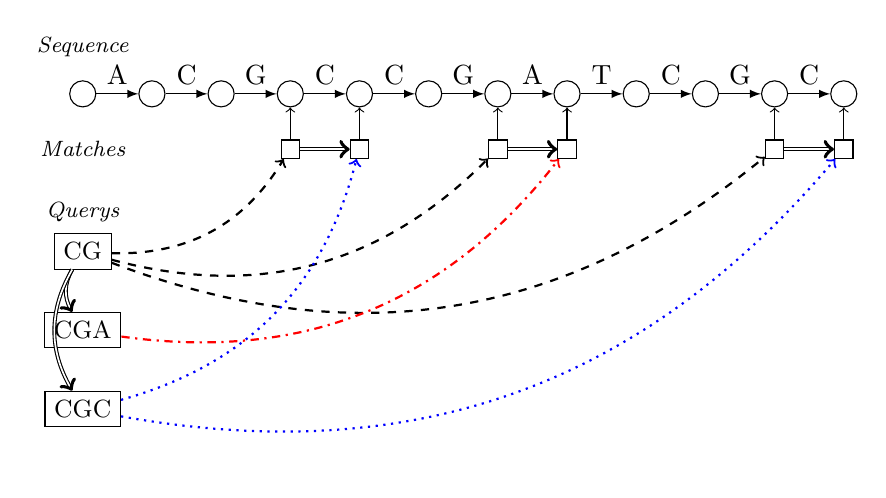
\begin{tikzpicture}[auto]
	\tikzstyle{state} = [ draw, circle, thin, node distance = 2.5em, font={\small}];
	\tikzstyle{query} = [ draw, rectangle, thin, node distance = 2.5em, font={\small}];
	\tikzstyle{info} = [font={\itshape\footnotesize}]
	\tikzstyle{point}  = [ ->, thin, font={\small}];
	\tikzstyle{extend} = [ ->, double, font={\small}];
	\tikzstyle{trace} = [ ->, thick, dashed, bend right, font={\small} ];

	\def \seq {X,A,C,G,C,C,G,A,T,C,G,C}

	\foreach \x [count=\xi] in \seq {
		\ifnum 1 < \xi
			\pgfmathparse{int(\xi-1)}
			\let \li \pgfmathresult
			\node[state, right of=\li] (\xi) {};
			\draw[->, >=latex] (\li) to node{\x} (\xi);
		\else
			\node[state] (\xi) {};
		\fi
	}

	\node[info] at (0,0.6) {Sequence};
	\node[info] at (0,-0.7) {Matches};
	\node[info] at (0,-1.5) {Querys};

	\node[query](CG)  at (0,-2) {CG};
	\node[query](CGA) at (0,-3) {CGA};
	\node[query](CGC) at (0,-4) {CGC};

	\tikzstyle{traceCG} = [ ->, thick, dashed, bend right, color=black ];
	\tikzstyle{traceCGA} = [ ->, thick, dashdotted, bend right, color=red ];
	\tikzstyle{traceCGC} = [ ->, thick, dotted, bend right, color=blue ];

	\draw[extend, bend right] (CG) to (CGA);
	\draw[extend, bend right] (CG) to (CGC);

	\foreach \xi/\xv in {4/CG,7/CG,11/CG} {
		\node[draw, below of=\xi, node distance=2em] (p\xi) {};
		\draw[point] (p\xi) to (\xi);
		\draw[trace\xv] (\xv) to (p\xi);
	}

	\foreach \xi/\xv in {5/CGC,8/CGA,12/CGC} {
		\node[draw, below of=\xi, node distance=2em] (p\xi) {};
		\draw[point] (p\xi) to (\xi);
		\draw[trace\xv] (\xv) to (p\xi);
	}

	\foreach \xi/\yi in {4/5,7/8,11/12} {
		\draw[extend] (p\xi) to (p\yi);
	}
\end{tikzpicture}

\end{figure}

Initially we have matches only for query $CG$. Then by taking the \emph{next} token from the sequence we can build up querys $CGA$ and $CGC$.

\subsection{Groups}

One common addition in a pattern language is capturing a group of tokens. For example we can use $X = [AC]$ to denote both tokens $A, C$. By adding where either one transitions we can capture such groups in the extension process.\

\begin{figure}[H]
	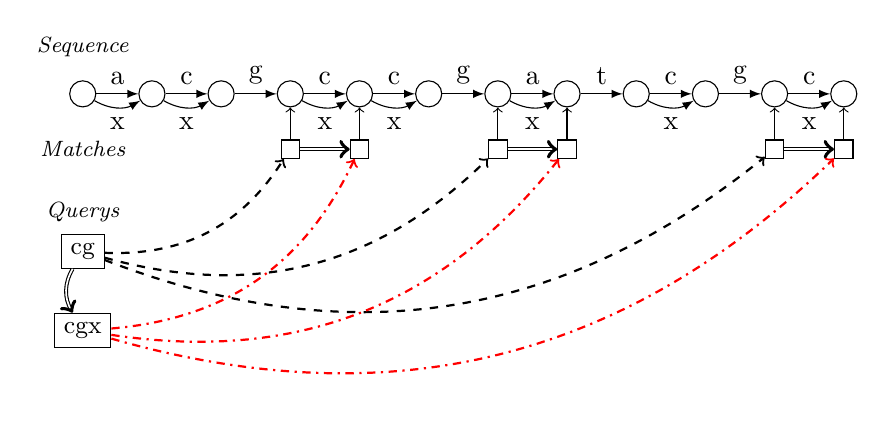
\begin{tikzpicture}[auto]
	\tikzstyle{state} = [ draw, circle, thin, node distance = 2.5em, font={\small}];
	\tikzstyle{query} = [ draw, rectangle, thin, node distance = 2.5em, font={\small}];
	\tikzstyle{info} = [font={\itshape\footnotesize}]
	\tikzstyle{point}  = [ ->, thin, font={\small}];
	\tikzstyle{extend} = [ ->, double, font={\small}];
	\tikzstyle{trace} = [ ->, thick, dashed, bend right, font={\small} ];

	\def \seq {x,a,c,g,c,c,g,a,t,c,g,c}

	\foreach \x [count=\xi] in \seq {
		\ifnum 1 < \xi
			\pgfmathparse{int(\xi-1)}
			\let \li \pgfmathresult
			\node[state, right of=\li] (\xi) {};
			\draw[->, >=latex] (\li) to node{\x} (\xi);
		\else
			\node[state] (\xi) {};
		\fi
	}

	\tikzstyle{exstate} = [ ->, bend right, >=latex];
	\foreach \xi/\yi in {1/2,2/3,4/5,5/6,7/8,9/10,11/12} {
		\draw[exstate] (\xi) to node[below]{x} (\yi);
	}


	\node[info] at (0,0.6) {Sequence};
	\node[info] at (0,-0.7) {Matches};
	\node[info] at (0,-1.5) {Querys};

	\node[query](cg)  at (0,-2) {cg};
	\node[query](cgx) at (0,-3) {cgx};

	\tikzstyle{tracecg} = [ ->, thick, dashed, bend right, color=black ];
	\tikzstyle{tracecgx} = [ ->, thick, dashdotted, bend right, color=red ];

	\draw[extend, bend right] (cg) to (cgx);

	\foreach \xi/\xv in {4/cg,7/cg,11/cg} {
		\node[draw, below of=\xi, node distance=2em] (p\xi) {};
		\draw[point] (p\xi) to (\xi);
		\draw[trace\xv] (\xv) to (p\xi);
	}

	\foreach \xi/\xv in {5/cgx,8/cgx,12/cgx} {
		\node[draw, below of=\xi, node distance=2em] (p\xi) {};
		\draw[point] (p\xi) to (\xi);
		\draw[trace\xv] (\xv) to (p\xi);
	}

	\foreach \xi/\yi in {4/5,7/8,11/12} {
		\draw[extend] (p\xi) to (p\yi);
	}
\end{tikzpicture}

\end{figure}

\subsection{Star}

Another possible extension is the \emph{dot-star} or more simply capturing a run of elements. Here we just show the expanded sequence with $*$ symbol.

\begin{figure}[H]
	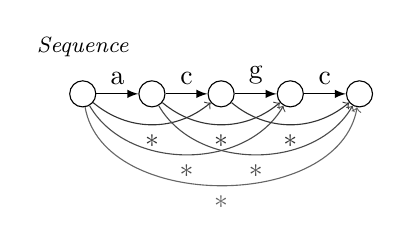
\begin{tikzpicture}[auto]
	\tikzstyle{state} = [ draw, circle, thin, node distance = 2.5em, font={\small}];
	\tikzstyle{query} = [ draw, rectangle, thin, node distance = 2.5em, font={\small}];
	\tikzstyle{info} = [font={\itshape\footnotesize}]
	\tikzstyle{point}  = [ ->, thin, font={\small}];
	\tikzstyle{extend} = [ ->, double, font={\small}];
	\tikzstyle{trace} = [ ->, thick, dashed, bend right, font={\small} ];

	\def \seq {x,a,c,g,c}

	\foreach \x [count=\xi] in \seq {
		\ifnum 1 < \xi
			\pgfmathparse{int(\xi-1)}
			\let \li \pgfmathresult
			\node[state, right of=\li] (\xi) {};
			\draw[->, >=latex] (\li) to node{\x} (\xi);
		\else
			\node[state] (\xi) {};
		\fi
	}

	\node[info] at (0,0.6) {Sequence};

	\tikzstyle{star} = [ ->, bend right, thin, color=black ];

	\foreach \xi in {1,...,3} {
		\pgfmathparse{int(\xi+2)}
		\let \xinext \pgfmathresult
		\foreach \yi in {\xinext,...,5} {
			\pgfmathparse{int(\yi - \xi)}
			\let \df \pgfmathresult
			\pgfmathparse{-\df*20}
			\let \out \pgfmathresult
			\pgfmathparse{int(180 - \out)}
			\let \in \pgfmathresult
			\pgfmathparse{int(100-\df*10)}
			\let \shade \pgfmathresult
			\draw[star, out=\out, in=\in, color=black!\shade] (\xi) to node[below]{$*$} (\yi);
		}
	}

\end{tikzpicture}

\end{figure}

Here we immediately notice how the complexity increases by introducing pattern token. \tow{properly} We can skip this intermediary step isn't necessary we can instead extend with $*Y$, where $Y$ is some other token. This means we avoid this single large query and have multiple smaller queries.

\begin{figure}[H]
	\begin{tikzpicture}[auto]
	\tikzstyle{state} = [ draw, circle, thin, node distance = 2.5em, font={\small}];
	\tikzstyle{query} = [ draw, rectangle, thin, node distance = 2.5em, font={\small}];
	\tikzstyle{info} = [font={\itshape\footnotesize}]
	\tikzstyle{point}  = [ ->, thin, font={\small}];
	\tikzstyle{extend} = [ ->, double, font={\small}];
	\tikzstyle{trace} = [ ->, thick, dashed, bend right, font={\small} ];


	\def \seq {X,A,C,G,C}

	\foreach \x [count=\xi] in \seq {
		\ifnum 1 < \xi
			\pgfmathparse{int(\xi-1)}
			\let \li \pgfmathresult
			\node[state, right of=\li] (\xi) {};
			\draw[->, >=latex] (\li) to node{\x} (\xi);
		\else
			\node[state] (\xi) {};
		\fi
	}

	\node[info] at (0,0.6) {Sequence};

	\tikzstyle{starC} = [ ->, bend right, thin, color=red ];
    \tikzstyle{starG} = [ ->, bend right, thin, color=blue ];

	\foreach \xi in {1,...,3} {
        \foreach \y [count=\yi] in \seq {
            \ifnumless{\xi+1}{\yi}{
                \pgfmathparse{int(\yi - \xi)}
                \let \df \pgfmathresult
                \pgfmathparse{-\df*20}
                \let \out \pgfmathresult
                \pgfmathparse{int(180 - \out)}
                \let \in \pgfmathresult

                \let \pat \seq[3]
                \draw[star\y, out=\out, in=\in] (\xi) to node[below]{$*$\y} (\yi);
            }
        }
	}

\end{tikzpicture}

\end{figure}

We can also limit the length of the run.

\begin{figure}[H]
	\begin{tikzpicture}[auto]
	\tikzstyle{state} = [ draw, circle, thin, node distance = 2.5em, font={\small}];
	\tikzstyle{query} = [ draw, rectangle, thin, node distance = 2.5em, font={\small}];
	\tikzstyle{info} = [font={\itshape\footnotesize}]
	\tikzstyle{point}  = [ ->, thin, font={\small}];
	\tikzstyle{extend} = [ ->, double, font={\small}];
	\tikzstyle{trace} = [ ->, thick, dashed, bend right, font={\small} ];


	\def \seq {X,A,C,G,C,C,G,A,T,C,G,C}

	\foreach \x [count=\xi] in \seq {
		\ifnum 1 < \xi
			\pgfmathparse{int(\xi-1)}
			\let \li \pgfmathresult
			\node[state, right of=\li] (\xi) {};
			\draw[->, >=latex] (\li) to node{\x} (\xi);
		\else
			\node[state] (\xi) {};
		\fi
	}

	\node[info] at (0,0.6) {Sequence};

	\tikzstyle{starC} = [ ->, bend right, thin, color=red ];
    \tikzstyle{starG} = [ ->, bend right, thin, color=blue ];
    \tikzstyle{starA} = [ ->, bend right, thin, color=green ];
    \tikzstyle{starT} = [ ->, bend right, thin, color=black ];

	\foreach \x [count=\xi] in \seq {
        \foreach \y [count=\yi] in \seq {
        	\pgfmathparse{int(\yi - \xi)}
            \let \df \pgfmathresult

            \ifnumcomp{1}{<}{\df}{
               	\ifnumcomp{\df}{<}{4}{
                	\pgfmathparse{-\df*20}
	                \let \out \pgfmathresult
	                \pgfmathparse{int(180 - \out)}
	                \let \in \pgfmathresult

	                \let \pat \seq[3]
	                \draw[star\y, out=\out, in=\in] (\xi) to node[below]{$*$\y} (\yi);
                }{}
            }{}
        }
	}

\end{tikzpicture}

\end{figure}

Here we have limited the run length to be either 2 or 3.

\subsection{Optimizations}

We can further optimize \emph{group next} by inferring the positions from simple \emph{sequence next}. We can see that the positions of a group extension is the same as the union of positions by the group tokens.

If we have a group token $\gamma$ that contains $tokens(\gamma)$ then the \emph{matches} for such group is $$matches(p\gamma, D) = \bigcup_{t \in tokens(\gamma)} matches(pt, D) $$


\section{Summary}

\tow{what follows, how used}